\documentclass[10pt]{article}
\usepackage{graphicx}
\usepackage{algorithm}
\usepackage{algpseudocode}

\begin{document}
\title{CSE616 Neural Networks and Their Applications\\
Project 1 Submission}
\author{Ayman Wagih Mohsen (2000728)}
\maketitle

\section{Introduction}
In this submission, we discuss and implement a variational autoencoder (VAE) based image compression technique. The VAE consists of an encoder and a decoder. The encoder generates mean and variance of latent space. The decoder reconstructs the image from latent space with transposed convolution.

\section{Dataset}
Due to computational resource constraints, we trained the autoencoder on the CIFAR10 dataset.

\section{Grouped Convolution}
We make use of convolution groups. As the data progresses from image space to latent space, the image resolution decreases, and the number of channels increases. Hence the convolution layers look more like fully connected layers. And since fully connected layers have too many learnable parameters (number of inputs times number of outputs), we divide the convolutions to isolated groups. This comes from the fact that the object details have a tree hierarchy. When we identify the broad class of an object, we are interested in the features of that class only. For example, there is no need to try to measure the wingspan of an object that was already identified earlier as a cat and not an airplane. Instead, we are interested in cat's ear size and eye color. We group the convolutions and increase the number of groups per layer as we progress from image space to latent space. This way we significantly save the number of filter weights as shown in the figure below.

\begin{center}
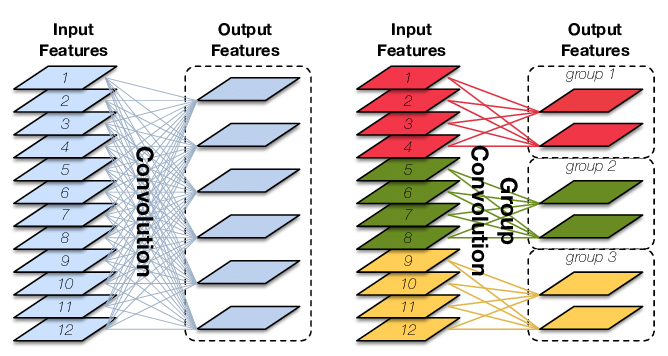
\includegraphics[width=0.9\textwidth]{grouped convolution.png}
\DeclareGraphicsExtensions{.png}
\end{center}

\section{Autoencoder operation}
At training time, the encoder tries to fit the mean and variance of the latent space. Then we sample random values from these normal distributions and pass them to the decoder. While at test time we use the mean value produced by the encoder as the latent code to compress. Before compressing the code it is quantized. To reflect this in the training process we add uniform quantization noise to the feature just before the mean and variance are calculated.

\section{Autoencoder versions}
We made two versions of the autoencoder. The first version had 136827 parameters (87612 in encoder and 49215 in decoder) and took over 60 training epochs to get acceptable results. While the second version has just 24075 parameters (15044 in encoder and 9031 in decoder) and took around 20 epochs to get acceptable results.

\begin{table}
\begin{tabular}{|l|l|l|l|l|l|}
Input & Filter & Stride & Pad & Output & Params\\
3*32*32		&1*12(3*4*4+1)		&1	&2	&1*12*16*16	&588\\
4*3*16*16	&4*12(3*4*4+1)		&1	&2	&4*12*8*8		&2352\\
16*3*8*8	&16*12(3*4*4+1)	&1	&2	&16*12*4*4	&9408\\
64*3*4*4	&64*12(3*4*4+1)	&1	&2	&64*12*2*2	&37632\\
64*3*4*4	&64*12(3*4*4+1)	&1	&2	&64*12*2*2	&3763\\
\end{tabular}
\caption{\label{tab:table-name}V1 Encoder shape. Note that the last two rows are repeated because each is used to get the mean and standard deviation of latent space at test time.}
\end{table}

\begin{table}
\begin{tabular}{|l|l|l|l|l|l|}
Input & Filter & Stride & Pad & Output & Params\\
64*12*2*2		&64*3(12*4*4+1)	&1	&2	&64*3*4*4		&37056\\
16*12*4*4		&16*3(12*4*4+1)	&1	&2	&16*3*8*8		&9264\\
4*12*8*8		&4*3(12*4*4+1)		&1	&2	&4*3*16*16	&2316\\
1*12*16*16	&1*3(12*4*4+1)		&1	&2	&1*3*32*32	&579\\
\end{tabular}
\caption{\label{tab:table-name}V1 Decoder shape.}
\end{table}

\begin{table}
\begin{tabular}{|l|l|l|l|l|l|}
Input & Filter & Stride & Pad & Output & Params\\
3*32*32		&1*12(3*6*6+1)		&2	&2	&1*12*16*16	&1308\\
4*3*16*16	&4*10(3*4*4+1)		&2	&2	&4*10*9*9	&1960\\
8*5*9*9		&8*16(5*3*3+1)		&2	&1	&8*16*5*5	&5888\\
8*5*9*9		&8*16(5*3*3+1)		&2	&1	&8*16*5*5	&5888\\
\end{tabular}
\caption{\label{tab:table-name}V2 Encoder shape. Note that the last two rows are repeated because each is used to get the mean and standard deviation of latent space at test time.}
\end{table}

\begin{table}
\begin{tabular}{|l|l|l|l|l|l|}
Input & Filter & Stride & Pad & Output & Params\\
8*16*5*5	&8*5(16*3*3+1)		&2	&1&	8*5*9*9		&5800\\
4*10*9*9	&4*3(10*4*4+1)		&2	&2	&4*3*16*16	&1932\\
1*12*16*16	&1*3(12*6*6+1)		&2	&2	&3*32*32		&1299\\
\end{tabular}
\caption{\label{tab:table-name}V2 Decoder shape.}
\end{table}

\begin{center}
\begin{figure}
\caption{Version 1 test results. Left: original images. Right: decoded images.}
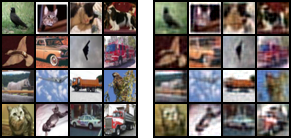
\includegraphics[width=0.9\textwidth]{20220530 1 v1.PNG}
\DeclareGraphicsExtensions{.png}
\end{figure}
\end{center}

\begin{center}
\begin{figure}
\caption{Version 2 test results. Left: original images. Right: decoded images.}
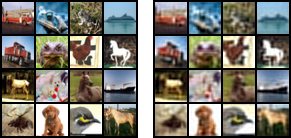
\includegraphics[width=0.9\textwidth]{20220530 2 v2.PNG}
\DeclareGraphicsExtensions{.png}
\end{figure}
\end{center}


\begin{thebibliography}{9}

\bibitem{paper1}
Johannes Ballé, Valero Laparra, Eero P. Simoncelli (2017) "End-to-end optimized image compression" https://arxiv.org/abs/1611.01704

\bibitem{paper2}
Jiaheng Liu, Guo Lu, Zhihao Hu, Dong Xu (2020) "A Unified End-to-End Framework for Efficient Deep Image Compression" https://arxiv.org/abs/2002.03370

\end{thebibliography}

\end{document}



